%% This is an example first chapter.  You should put chapter/appendix that you
%% write into a separate file, and add a line \include{yourfilename} to
%% main.tex, where `yourfilename.tex' is the name of the chapter/appendix file.
%% You can process specific files by typing their names in at the 
%% \files=
%% prompt when you run the file main.tex through LaTeX.

\chapter{Case Studies}\label{Chap:CaseStudies}

This chapter presents three case studies used to evaluate \sys{}. Each case study involves using \sys{} on a web service that is unique in some fundamental way. This variability stress tests \sys{}'s two main objectives: minimal intrusiveness and ease of configuration. The case studies provide guidance on what aspects of \sys{} need configuration and precisely how detailed versus general those configurable options should be to be beneficial without becoming overly burdensome.

\section{Conduit}

Conduit is a simple RESTful blog web service~\cite{conduit}. It is not a production service, rather an educational service to demonstrate the flexibility of RESTful web applications. The project supplies many simple frontend and backend implementations, written in various programming languages and frameworks, but following the same API. The case study focused on a React based frontend~\cite{conduit-frontend} and a Golang based backend~\cite{conduit-backend}. Conduit is the best-case application for the WebAuthn firewall, a RESTful web service with basic functionality to protect. No backend modifications are necessary to integrate WebAuthn.

%% 
%% \iffalse
%% This way, they can be interchanged without problem. 
%% \fi
%% 

%% \subsubsection{User Identification}
%% TODO: Maybe talk about JWT

\subsection{Context Retrieval}\label{Sec:Conduit_ContextRetrieval}

A major benefit of a RESTful web application is that the backend exposes many useful context routes. By design, a RESTful frontend performs the necessary rendering on the user's web-browser and must retrieve user specific information from the backend. These routes are useful for WebAuthn context retrieval as well. For example, the backend already implements routes such as getting an article by its ID. And if not, then there certainly will be a tangential route such as requesting all comments of an article to search for a specific one by ID. Since most of the modifications necessary to the backend when integrating the WebAuthn firewall are for context routes, this aspect of RESTful applications make that easy.

\subsection{Secured Routes}

The Conduit case study has three protected routes. Table~\ref{Table:ConduitSecuredRoutes} lists the secured operations with a sample authentication message for each. It presents an overview of how Conduit is protected with transaction authentication.

\begin{table}[h]
\centering

\begin{tabular}{ m{5cm} m{9cm}  } 
 \hline
 Operation & Authentication Message \\ 
 \hline \hline

 Delete Comment & \lstinline|"Confirm comment delete: I love WebAuthn"| \\ \hline

 Delete Article & \lstinline|"Confirm article delete: Cat Memes"| \\ \hline

 Update User Settings & 
%% TODO: Figure out how to remove numbering and frame
 \begin{lstlisting} 
"Confirm new user details:
   username damian
   email damianb@mit.edu"
\end{lstlisting} 
\\ \hline

\end{tabular}
\caption{The operations of Conduit secured by transaction authentication.}
\label{Table:ConduitSecuredRoutes}
\end{table}

The simplicity of the Conduit application does not challenge the domain specific language much. The domain specific programs simply retrieve some context to complete the format strings. The ``Update User Settings'' route requires a custom handler, which is not exceptionally complicated. The custom handler transaction authenticates requests only if the username, email or password are modified. Otherwise, HTTP requests that only modify non-sensitive fields like the bio or profile pictures pass through without any verification.

%% 
%% \iffalse
%% Otherwise, HTTP requests to modify only the bio or profile pictures pass through without any verification.
%% \fi
%% 

\section{Calypso}

Calypso is a RESTful frontend for a WordPress admin panel~\cite{calypso}. This is a production service, with far greater complexity than the Conduit application. Also, unlike Conduit with a backend running locally, which can be modified, Calypso accesses the official WordPress backend servers. These servers are closed-source and their modification is out of question. Whereas avoiding backend modifications for Conduit is a favorable result, with Calypso it is a necessity. Nonetheless, integrating WebAuthn is possible because the RESTful API of WordPress was complete enough to satisfy the needs of \sys{}.

\subsection{Multi-Target Proxying}

\begin{figure}[h]
  \centering
  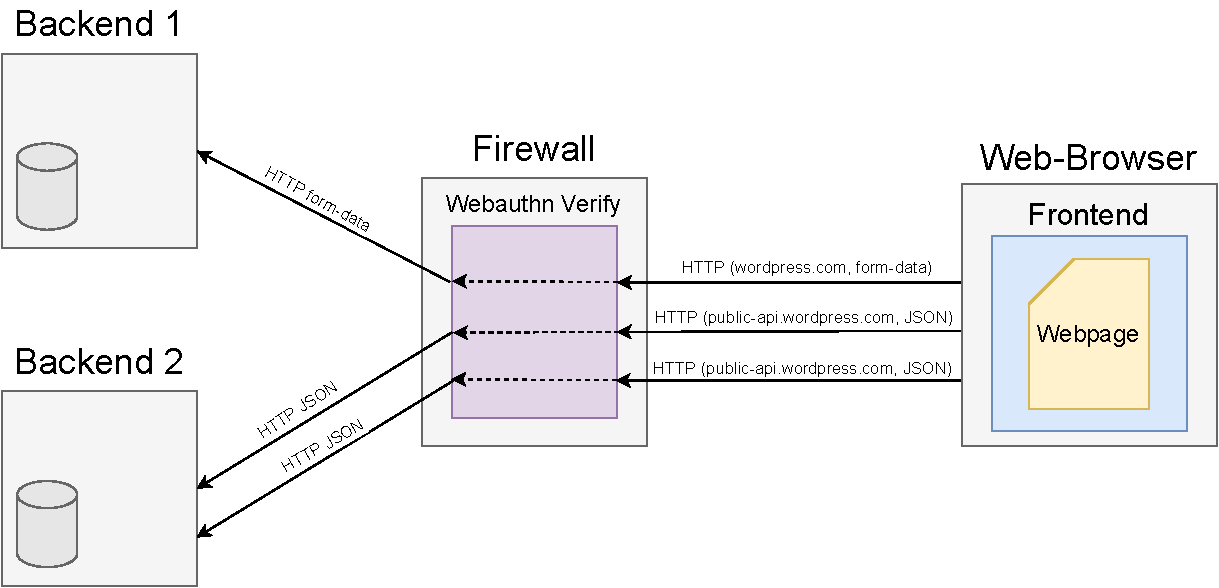
\includegraphics[width=14cm]{multitarget_calypso_drawio}
  \caption{The WebAuthn firewall must support two backend targets for Calypso.}
  \label{Fig:MultiTargetCalypso}
\end{figure}

%% 
%% \iffalse
%% Requests sent to the firewall contain their destined targets in their headers, and the firewall proxies accordingly. 
%% \fi
%% 

Unlike the other two case studies, a point of complexity that Calypso has is that the frontend accesses multiple backends. Typically, the frontend requests to a single backend source. However, as shown in Figure~\ref{Fig:MultiTargetCalypso}, the Calypso frontend interfaces with two backend targets. \sys{} receives requests with target addresses \lstinline{"public-api.wordpress.com"} and \lstinline{"wordpress.com"} in their headers. It must proxy them to their respective backends accordingly. One WordPress backend is for API requests located at \lstinline{"public-api.wordpress.com"} and accepts JSON payloads. Most of Calypso interacts with this backend. However, login requests go to a backend at \lstinline{"wordpress.com"} which uses form-data payloads. This architecture design requires that \sys{} support multi-target proxying with separate default input getter functions per target. The firewall configuration for Calypso lists both of those target domains along with \lstinline{GetJSONInput} and \lstinline{GetFormInput} as their default input handlers respectively. 

\subsection{Login}\label{Sec:CalypsoLogin}

\sys{} transparently protects a number of core WebAuthn routes, including the route for login, as described in Section~\ref{Sec:DefaultHandlers}. However, the Calypso project approaches login in an atypical fashion. Normally a service has a dedicated route for login. Calypso shares a login route with other operations, so HTTP requests are identified by an \lstinline{"action"} field in their payload, similarly as described in Section~\ref{Sec:CustomHandlers}. As a result, the default login handler cannot support Calypso directly. Extending the default login handler to be customizable for this one specific case would make \sys{}'s configuration too complicated. Rather, a custom login handler implements the Calypso login event. The login handler roughly resembles the Go pseudo-code in Code Snippet~\ref{code:finishLogin}.

\begin{lstlisting}[float=h,label=code:finishLogin,caption=Go pseudo-code for the custom login handler for Calypso.]
func finishLogin(w http.ResponseWriter, req *wf.ExtendedRequest) {
  action := req.Get("action")
  switch action {
    case "login-endpoint":
      // WebAuthn verify the login request
      VerifyLogin(w, req)
    default:
      // Other requests go right through
      ProxyRequest(w, req)
  }
}
\end{lstlisting}

The handler listens on the \lstinline{"wordpress.com/wp-login.php"} route. It extracts the \lstinline{"action"} field in the request payload and validates the login attempt only if the action is \lstinline{"login-endpoint"}. The \lstinline{VerifyLogin} function performs the WebAuthn authentication and only upon successful verification does it allow the request to proceed through the firewall. Otherwise, all other requests are proxied through with no additional checks.

\subsection{Secured Routes}\label{Sec:CalypsoSecuredRoutes}

Table~\ref{Table:CalypsoSecuredRoutes} lists the secured operations of Calypso with a sample authentication message for each. The domain specific language supports Calypso well; every operation listed is secured using the domain specific language. This array of protected operations demonstrates the flexibility of the domain specific language.

\begin{table}[h]
\centering

\begin{tabular}{ m{5cm} m{9cm}  } 
 \hline
 Operation & Authentication Message \\ 
 \hline \hline

 Update Profile Settings & \lstinline|"Save the profile settings: Espanol Public"| \\ \hline

 Invite New Users to Site & \lstinline|"Invite new users: damian, durian, john-smithson"| \\ \hline

 Change Site Address & 
%% TODO: Figure out how to remove numbering and frame
 \begin{lstlisting} 
"Change site address
   from: calypso.localhost
   to: mytravels.blog.com"
\end{lstlisting} 
\\ \hline

 Change Site Theme & \lstinline|"Change theme to: Tangerine Orange"| \\ \hline

\end{tabular}
\caption{The operations of Calypso secured by transaction authentication.}
\label{Table:CalypsoSecuredRoutes}
\end{table}

Certain domain specific programs have multiple context retrievals. Others have multiple format tags to fill, and one program requires a special formatting function. Apart from the custom login handler, there is no case where a custom handler is necessary. 
The ``Invite New Users to Site'' route receives HTTP request containing an array of elements that must be comma separated in the authentication message. Rather than implementing a custom handler for this minor inconvenience, the \lstinline{Apply} domain specific operation described in Table~\ref{Table:DSL_GetterOperations} resolves this problem. It enables Go code to be used within a domain specific program to a limited extent. Code Snippet~\ref{code:inviteNewUsersDSL} is a domain specific program for inviting new users to administer a WordPress blog.

%% 
%% \iffalse
%% all of the routes in Calypso are protected using the DSL. 
%% \fi
%% 

\begin{lstlisting}[float=h,label=code:inviteNewUsersDSL,caption=A domain specific program to secure the Calypso operation for inviting new users to administer a WordPress blog.]
Secure("POST", "/rest/{version}/sites/{site_id}/invites/new", 
  Authn("Invite new user(s): %v",
    wf.Apply(func(args ...interface{}) (interface{}, error) {
      invitees := args[0].([]string)
      return strings.Join(invitees, ","), nil
    }, wf.GetArray("invitees")),
))
\end{lstlisting}

The \lstinline{Authn} operation string formats the argument of \lstinline{wf.GetArray("invitees"))} with a Go closure passed to \lstinline{Apply}.

\section{Gogs}

Gogs is a server-side rendered self-hosted Git web service~\cite{gogs}. A server-side rendered web application presents its own set of challenges to the WebAuthn firewall. Section~\ref{Sec:ProxyingRequests} explains how \sys{} has to be the end-point interacting with the user's web-browser. The firewall must obtain the context from the Gogs backend. The backend does not, however, conveniently expose context routes like RESTful backends as discussed in Section~\ref{Sec:Conduit_ContextRetrieval}.

%% 
%% \iffalse
%% Apart from that, context must be served by the Gogs backend. 
%% \fi
%% 

\subsection{Intrusive WebAuthn}

The Gogs web service was the first of the three case-studies. Before \sys{} became a mature idea, part of Gogs was secured in the traditional, intrusive fashion described in Section~\ref{Sec:StatusQuo}. This work is redone using the WebAuthn firewall approach once it proved itself as a prospective design approach.

The two main challenges with integrating WebAuthn into Gogs intrusively are the database adapter and organizational difficulties. WebAuthn needs a database table to record entries of users' public key credentials. Simply creating a new table in Gogs requires writing a custom database model for the table as well as modifying the codebase in a number of separate locations. Furthermore, the handlers for various Gogs routes are spread throughout the code. Keeping track of which routes are WebAuthn secured becomes increasingly more difficult as more routes are protected.

%% 
%% \iffalse
%% The intrusive approach was abandoned once the firewall proved itself a prospective mechanism and all of the work redone.
%% \fi
%% 

\subsection{Context Retrieval}

A downside to server-side rendering web services when compared to RESTful services when it comes to WebAuthn firewall integration is the lack of pre-built context routes. Effectively, the API routes in the RESTful backend services act as the context routes. Gogs, being a server-side rendering backend, must be modified to include those context routes. Some Gogs routes need additional context to retrieve objects such as a \lstinline{"repository"} or \lstinline{"webhook"}. Gogs serves this context information out of a \lstinline{"server_context/<type>/<args>"} route. The \lstinline{<type>} refers to what type of object is being requested (e.g., repository, webhook, etc.). Each context type has its own handler in Gogs, which interprets the \lstinline{<args>} to retrieve the correct context object.

%% 
%% \iffalse
%% As the Gogs routes get webauthn protected, becomes more evident which 
%% \fi
%% 

\subsection{Secured Routes}

While integrating WebAuthn into Gogs during the case study, every HTTP route of the web service is categorized whether it should be protected by transaction authentication or not. This judgment is made by weighing the cost versus the benefit of protecting that route. Protecting a route is not free, most heavily affecting the user experience. Routes are protected if the harm due to malicious hijacking justifies the burden to the user's experience.

Table~\ref{Table:GogsSecuredRoutes} lists the secured operations with a sample authentication message for each. It presents an overview for the types of operations that could warrant WebAuthn transaction authentication.

\begin{table}[h]
\centering

\begin{tabular}{ m{5cm} m{9cm}  } 
 \hline
 Operation & Authentication Message \\ 
 \hline \hline

 Delete Repository & \lstinline|"Confirm repository delete: damian/JS-OS"| \\ \hline

 Add SSH Key & \lstinline|"Add SSH key named: Damian's Laptop"| \\ \hline

 Delete SSH Key & \lstinline|"Delete SSH key named: Damian's Laptop"| \\ \hline

 Update Profile Settings & 
%% TODO: Figure out how to remove numbering and frame
 \begin{lstlisting} 
"Confirm profile details:
   username damian
   email damianb@mit.edu"
\end{lstlisting} 
\\ \hline

 Set Primary Email & \lstinline|"Confirm new primary email: damianb@alum.mit.edu"| \\ \hline

 Change Password & \lstinline|"Confirm password change"| \\ \hline

 Leave Repository & \lstinline|"Leave repository named: JS-OS"| \\ \hline

 Delete App Access Token & \lstinline|"Delete App named: Gogs-Watcher-App"| \\ \hline

 Publish New Release &
%% TODO: Figure out how to remove numbering and frame
 \begin{lstlisting} 
"Publish release named: Version 4.20
   File names: release.tar.gz, release"
\end{lstlisting} 
\\ \hline

  Delete Web-Hook & \lstinline|"Delete webhook for: URL gogswatcher.app.com"| \\ \hline

\end{tabular}
\caption{The operations of Gogs secured by transaction authentication.}
\label{Table:GogsSecuredRoutes}
\end{table}

\subsection{Custom Handlers}\label{Sec:Gogs_CustomHandlers}

As with the other case-studies, most of the routes are simple and easy to secure using the domain specific language. At most they require a context retrieval to fill a single format tag. Within the Gogs service, the ``Delete Repository'' and ``Set Primary Email'' operations in Table~\ref{Table:GogsSecuredRoutes} are handled by HTTP routes that also handle multiple other operation types. Similarly to the login route of Calypso discussed in Section~\ref{Sec:CalypsoLogin}, requests have an \lstinline{"action"} field in their payload that delineates the operation type. Only certain actions warrant being transaction authenticated. Custom handlers are used in these cases, to parse the \lstinline{"action"} field and WebAuthn secure only when necessary.

 %% 
%% \iffalse
%% each share the same HTTP route for multiple different HTTP operations. 

%% there are a number of routes such as the ``Delete Repository'' that are shared by multiple HTTP operations.

%% publishing a new release. 
%% \fi
%% 

Gogs requires a more involved custom handler for protecting the ``Publish New Release'' operation. The files associated with a new release are contained as UUIDs in the HTTP request. So each file needs context retrieval to retrieve the file name, which then must be comma separated in the format string. Rather than expressing this series of operations and formatting in an \lstinline{Apply} operation like with Calypso in Section~\ref{Sec:CalypsoSecuredRoutes}, it is easier to drop down to a custom handler function. The custom handler function written in Go pseudo-code is produced in Code Snippet~\ref{code:publishNewRelease}.

\begin{lstlisting}[float=h,label=code:publishNewRelease,caption=A custom handler in Go pseudo-code to secure the Gogs operation for publishing a new release.]
func publishNewRelease(w http.ResponseWriter, 
                       r *wf.ExtendedRequest) {
  title := r.Get("title")
  uuids := r.Request.Form["files"]

  names := []string{}
  for _, uuid := range uuids {
    append(names, r.GetContext("attachment", uuid)["Name"].(string))
  }

  authText := fmt.Sprintf("Publish release named: %v", title)
  authText += fmt.Sprintf("\nFile names: %s", 
                          strings.Join(names, ", "))

  handlerFn := firewall.Authn(authText)
  handlerFn(w, r)
}
\end{lstlisting}

This handler constructs an authentication message from the \lstinline{"title"} of the release and all of the included attachment file names. For the attachment file names, the handler must translate the UUIDs into contextualized attachment objects and then look up the \lstinline{"Name"} fields.

%% 
%% \iffalse
%% Essentially, the firewall assumes the roles of the frontend in the RESTful use-cases. 

%% of the \lstinline{"Name"} fields for every attachment UUID of the new relase
%% \fi
%% 
